%===================================================================================
% JORNADA CIENTÍFICA ESTUDIANTIL - MATCOM, UH
%===================================================================================
% Esta plantilla ha sido diseñada para ser usada en los artículos de la
% Jornada Científica Estudiantil de MatCom.
%
% Por favor, siga las instrucciones de esta plantilla y rellene en las secciones
% correspondientes.
%
% NOTA: Necesitará el archivo 'jcematcom.sty' en la misma carpeta donde esté este
%       archivo para poder utilizar esta plantila.
%===================================================================================



%===================================================================================
% PREÁMBULO
%-----------------------------------------------------------------------------------
\documentclass[a4paper,10pt,twocolumn]{article}

%===================================================================================
% Paquetes
%-----------------------------------------------------------------------------------
\usepackage{amsmath}
\usepackage{amsfonts}
\usepackage{amssymb}
\usepackage{jcematcom}
\usepackage[utf8]{inputenc}
\usepackage{listings}
\usepackage[pdftex]{hyperref}
\usepackage{caption}
\usepackage{subcaption}
%-----------------------------------------------------------------------------------
% Configuración
%-----------------------------------------------------------------------------------
\hypersetup{colorlinks,%
	    citecolor=black,%
	    filecolor=black,%
	    linkcolor=black,%
	    urlcolor=blue}

%===================================================================================



%===================================================================================
% Presentacion
%-----------------------------------------------------------------------------------
% Título
%-----------------------------------------------------------------------------------
\title{Identificando Elenas (\textit{Eleutherodactylus eileenae}) a partir de audios desordenados}

%-----------------------------------------------------------------------------------
% Autores
%-----------------------------------------------------------------------------------
\author{\\
\name Daniel Machado Pérez \email \href{mailto:daniel.machado@gmail.com}{daniel.machado@gmail.com}
	\\ \addr Grupo C411}

%-----------------------------------------------------------------------------------
% Tutores
%-----------------------------------------------------------------------------------
\tutors{\\
Dr. Roberto Mulet, \emph{Facultad de Física}}

%-----------------------------------------------------------------------------------
% Headings
%-----------------------------------------------------------------------------------
\jcematcomheading{\the\year}{1-\pageref{end}}{D. Machado}

%-----------------------------------------------------------------------------------
\ShortHeadings{Identificando Elenas (\textit{Eleutherodactylus eileenae})}{Daniel Machado Pérez}
%===================================================================================



%===================================================================================
% DOCUMENTO
%-----------------------------------------------------------------------------------
\begin{document}

%-----------------------------------------------------------------------------------
% NO BORRAR ESTA LINEA!
%-----------------------------------------------------------------------------------
\twocolumn[
%-----------------------------------------------------------------------------------

\maketitle

%===================================================================================
% Resumen y Abstract
%-----------------------------------------------------------------------------------
\selectlanguage{spanish} % Para producir el documento en Español

%-----------------------------------------------------------------------------------
% Resumen en Español
%-----------------------------------------------------------------------------------
\begin{abstract}


Este estudio analiza las secuencias de cantos de la 
rana \textit{Eleutherodactylus eileenae} (que llamaremos Elena), 
obtenidos mediante grabaciones de campo realizadas 
con nueve micrófonos distribuidos alrededor de los 
especímenes. Para identificar las secuencias 
probables de los cantos se propone un método que 
emplea mel-espectrogramas y análisis de las energías 
temporales de las grabaciones. Para garantizar la sincronización de 
los audios, se procedió con la obtención de
los momentos de pico de energía y el cálculo de los 
desfases con correlación cruzada utilizando un 
archivo de referencia. Cada canto es conocido comúnmente como
Colín, en imitación al sonido producido, en el que se emite
una señal con frecuencia baja que denominaremos CO y una con frecuencia
alta que llamaremos LIN. Los resultados 
revelan patrones en la estructura del coro, donde 
cada rana parece mantener una periodicidad consistente 
entre cantos y ajustar las frecuencias en respuesta a 
otros individuos.
	
	

\end{abstract}

%-----------------------------------------------------------------------------------
% English Abstract
%-----------------------------------------------------------------------------------
\vspace{0.5cm}

\begin{enabstract}

	This study analyzes the call sequences of the 
	frog \textit{Eleutherodactylus eileenae} 
	(which we will refer to as Elena), 
	obtained through field recordings made with 
	nine microphones placed around the specimens. 
	To identify the probable call sequences, 
	a method is proposed that uses mel-spectrograms 
	and temporal energy analysis of the recordings. 
	To ensure the synchronization of the audios, 
	the energy peak moments were obtained, 
	and the time lags were calculated using 
	cross-correlation with a reference file. 
	Each call is commonly known as Colín, 
	imitating the sound produced, 
	where a signal with a low frequency, called CO, 
	and a high frequency, called LIN, is emitted. 
	The results reveal patterns in the structure of 
	the chorus, where each frog seems to maintain a 
	consistent period between calls and adjust its 
	frequencies in response to other individuals.
\end{enabstract}

%-----------------------------------------------------------------------------------
% Palabras clave
%-----------------------------------------------------------------------------------
\begin{keywords}
	Elena,
	Energía Temporal,
	Frecuencia,
	Mel-Espectrograma,
	Colín,
	Correlación Cruzada.
\end{keywords}

%-----------------------------------------------------------------------------------
% Temas
%-----------------------------------------------------------------------------------
\begin{topics}
	Sistemas Computacionales, Procesamiento y Análisis de Señales.
\end{topics}


%-----------------------------------------------------------------------------------
% NO BORRAR ESTAS LINEAS!
%-----------------------------------------------------------------------------------
\vspace{0.8cm}
]
%-----------------------------------------------------------------------------------


%===================================================================================

%===================================================================================
% Resumen Extendido
%-----------------------------------------------------------------------------------
\section{Resumen Extendido}\label{sec:intro}
%-----------------------------------------------------------------------------------
  
\textbf{Breve Resumen del Estado del Arte}\\

El estudio de las señales acústicas en animales 
para distinguir individuos y analizar su 
comportamiento ha evolucionado considerablemente. 
\href{https://besjournals.onlinelibrary.wiley.com/doi/full/10.1111/j.1365-2664.2011.01993.x}{Blumstein et al. (2011)} propusieron el uso de arreglos 
de micrófonos para la detección y localización de 
fuentes acústicas, destacando el potencial de las 
correlaciones cruzadas para diferenciar individuos. 
En el campo de la ecoacústica, \href{https://www.mdpi.com/2227-7390/7/1/21}{Farina (2018)} introdujo 
técnicas y métricas para caracterizar estructuras de 
coro y patrones de comportamiento, abriendo nuevas 
áreas de análisis en bioacústica. 
Akmentins (\href{https://www.tandfonline.com/doi/abs/10.1080/00222933.2011.560967}{2011}, \href{https://www.tandfonline.com/doi/abs/10.1080/09524622.2014.965217}{2015}) implementó dispositivos de 
grabación automatizados y técnicas de clasificación 
mediante transformadas de Fourier para identificar 
especies y tipos de vocalización en ranas. 
En años recientes, se han desarrollado métodos de 
clasificación de coros mediante espectrogramas, 
como los trabajos de \href{https://www.sciencedirect.com/science/article/pii/S2666827021001018}{Xie et al. (2022)} y \href{https://www.sciencedirect.com/science/article/abs/pii/S1574954120301102}{Gan et al. (2020)}, 
quienes emplearon redes neuronales y algoritmos de 
aprendizaje automático para detectar coros en 
condiciones ambientales diversas. 
Recientemente, investigaciones como las de 
\href{https://onlinelibrary.wiley.com/doi/abs/10.1111/ele.14002}{Calsbeek et al. (2022)} y \href{https://www.sciencedirect.com/science/article/abs/pii/S1574954117300201}{Sánchez-Gendriz y Padovese (2017)} 
han explorado las dinámicas de coro y la elección sexual, 
logrando avances en la caracterización individual de 
los sonidos en especies de ranas mediante análisis de 
niveles de presión sonora y técnicas de filtrado. 
Sin embargo, hasta la fecha, no se ha propuesto un 
método automático para discriminar individuos dentro 
de un coro utilizando exclusivamente arreglos de 
micrófonos.\\

\textbf{Problema Tratado}\\


La rana \textit{Eleutherodactylus eileenae} (Elena)  
es una especie endémica de Cuba \cite{elena}. 
Su canto (Colín) es característico y se compone de dos 
partes: una señal con frecuencia baja que 
denominaremos CO y una con frecuencia alta que 
llamaremos LIN. Estas señales se emiten en 
secuencias que se repiten a lo largo del tiempo, 
formando un coro.\\

La Elena es una especie estudiada por profesores e investigadores
de la Facultad de Biología de la Universidad de La Habana. Como parte de sus
investigaciones, fue planteada la necesidad de analizar el comportamiento de los 
coros antes mencionados. Se quiere saber si poseen una estructura determinada,
si existen individuos que juegan un papel protagónico, entre otras cosas. 
Hasta el momento, el procesamiento de la información recopilada se realizaba manualmente,
por lo que, para provocar avaces más eficientes y rigurosos en los estudios,
se impone la automatización de estos procesos y su trato con un enfoque más 
computacional.\\

El objetivo de este estudio es 
estudiar dichos coros, por lo que la primera tarea que se planteó fue la de
identificar las secuencias probables de los cantos de 
Elena a partir de grabaciones de campo realizadas con 
nueve micrófonos distribuidos alrededor de los 
especímenes. Como los micrófonos están ubicados
relativamente cercanos, cada uno capta los cantos de más de una rana. 
De ahí surge la necesidad de un método para distinguir los cantos
del espécimen más cercano a cada dispositivo para, una vez hecho esto, conformar
las secuencias generales. Para visualizar la distribución geográfica de los 
micrófonos véase la Figura \ref{fig:mics}

\begin{figure}[h!]
    \centering
    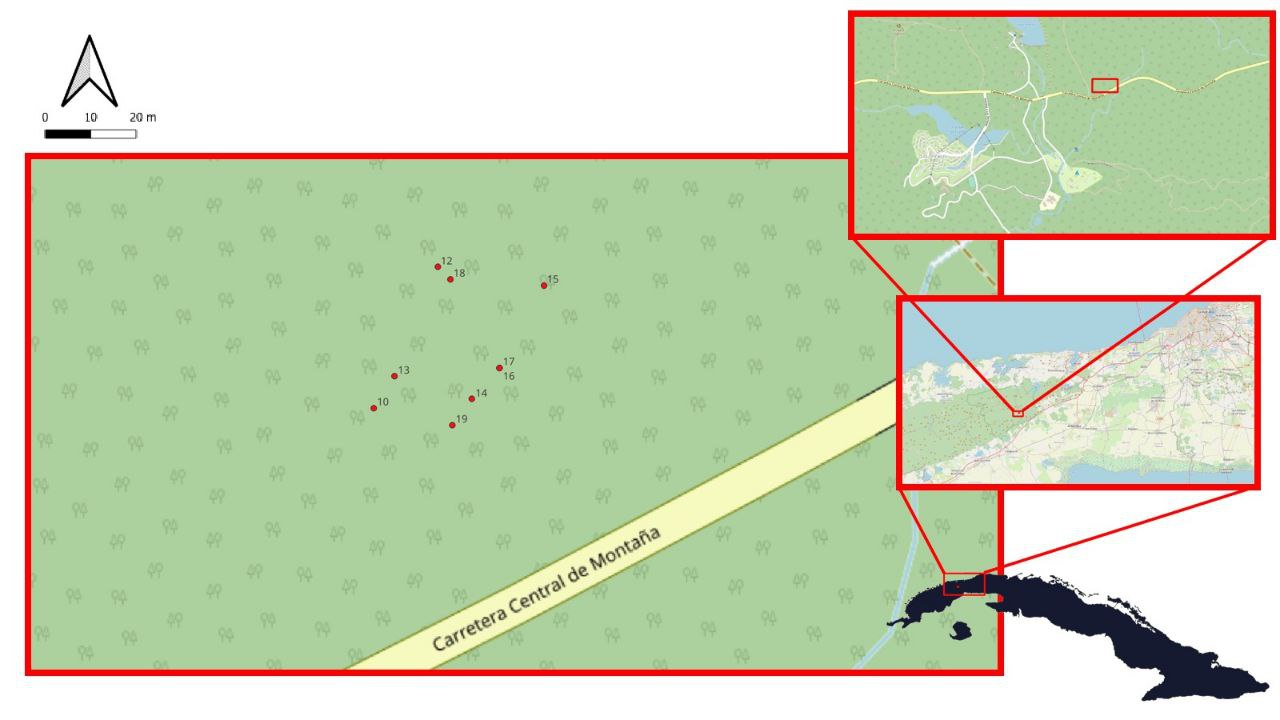
\includegraphics[width=\columnwidth]{assets/mic_map.jpg}
    \caption{Distribución Geográfica de los Micrófonos.}
    \label{fig:mics}
\end{figure}

Se cuenta con el \textit{dataset} de las grabaciones hechas por los 9 micrófonos. 
Estas se realizaron durante 3 días, a partir de las 18:00 hasta las 06:00 horas del día siguiente,
donde de cada hora se registraron 58 minutos y se descansaron 2. 
Los dispositivos se activaron remotamente y al mismo tiempo. 
Para lo que se expone en el presente informe, se utilizó la información
captada el día 21 de octubre de 2023 a las 19:00 horas.
En gran parte de la investigación se trabajará cada audio como el mel-espectrograma 
correspondiente \cite{mel}. Los parámetros utilizados para la obtención de cada uno fueron los siguientes:

\begin{itemize}
	\item hop\_length: 512
	\item n\_fft: 6096
	\item n\_mels: 128
	\item f\_min: 1600
	\item f\_max: 4096
	\item sample\_rate: 96000
\end{itemize}

Para mayor facilidad en el tratamiento de los archivos y su fácil distinción, fueron 
renombrados para asignarle a cada uno de los 9 audios una letra de la \textbf{a} a la \textbf{i}.
En la Figura \ref{fig:mel} se puede observar un ejemplo de mel-espectrograma de un fragmento del audio \textbf{h}
a la hora y el día seleccionados.

\begin{figure}[h!]
    \centering
    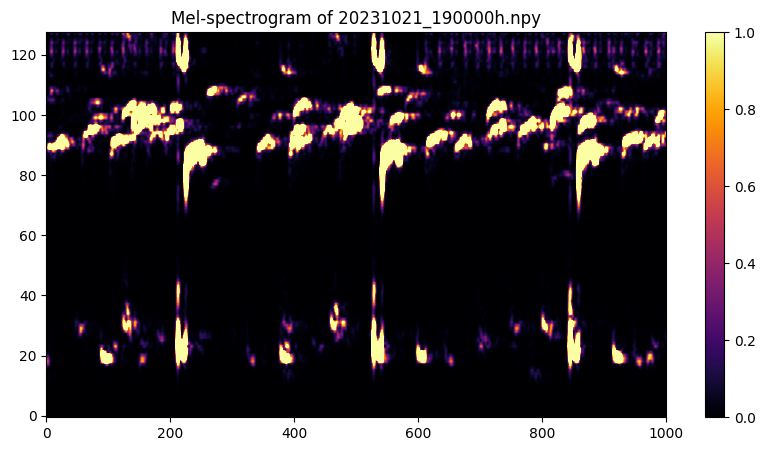
\includegraphics[width=\columnwidth]{assets/mel-spectrogram.png}
    \caption{Ejemplo de Mel-Espectrograma de Fragmento del Audio \textbf{h}.}
    \label{fig:mel}
\end{figure}

Previo al estudio que fue propuesto, es necesario preprocesar los archivos de audio. 
Fundamentalmente se debe garantizar un alto grado de sincronización.
A pesar de que las grabaciones comenzaron a la misma hora, existe un \textit{lag} no 
despreciable entre ellas, cosa que perjudica el análisis en cuestión. 
Para corregir dicho error se diseñó un proceso semi-automático que se sustenta
en el método conocido de \textbf{Correlación Cruzada} \cite{cross_corr}. El plan consiste en 
la alineación de los archivos con base en un pivote que debe ser seleccionado.
Esto se lleva a cabo mediante el cálculo de las energías temporales a partir de los mel-espectrogramas,
la identificación de los momentos de pico de energía, la aplicación de \textbf{Correlación Cruzada} y 
la corrección de los desfases.\\


El proceso detallado de sincronización sigue los siguientes pasos:\\


\textbf{Selección de un rango de bandas de frecuencia y un pivote.}\\

Para ello se recomienda identificar un archivo en el que sea distinguible
una señal (ya sea de CO o de LIN) que resalte en cuanto a intensidad,
presencia en todos los archivos, y `limpieza', queriendo indicar con
esta último aspecto que en el rango de bandas de frecuencia en que se encuentra
no exista un elevado número de otras señales que puedan constituir ruido
y `ensuciar' la información. El audio donde dicha señal se manifiesta
con mayor claridad y/o intensidad puede ser seleccionado como pivote.
Mientras tanto el rango de bandas de frecuencia que contenga la señal y minimice
el ruido puede ser el indicado para la sincronización. A partir de esa selección,
el proceso restante se realiza con la información filtrada.\\

Por ejemplo, en el dataset que se usará para mostrar los resultados de este trabajo, 
se seleccionó como pivote al audio \textbf{h} y el rango de bandas de frecuencia de 113 a 117,
por las características distintivas que se observan en la Figura \ref{fig:mel}.\\

\textbf{Cálculo de las energías temporales de cada archivo.}\\

En cada instante de tiempo, la energía se calcula de la siguiente forma:\\

\begin{equation*}
	E_j = \sum_{i=0} a_{ij}^{2}, \forall j     \cite{energy}
\end{equation*} 


donde:\\
$E_j$ es la energía en el instante de tiempo $j$,\\
$a_{ij}$ es la intensidad en el instante de tiempo $j$ y la banda de frecuencia $i$.\\

Para el audio \textbf{h}, su energía temporal se puede visualizar en la gráfica de la Figura \ref{fig:energy}\\

\begin{figure}[h!]
    \centering
    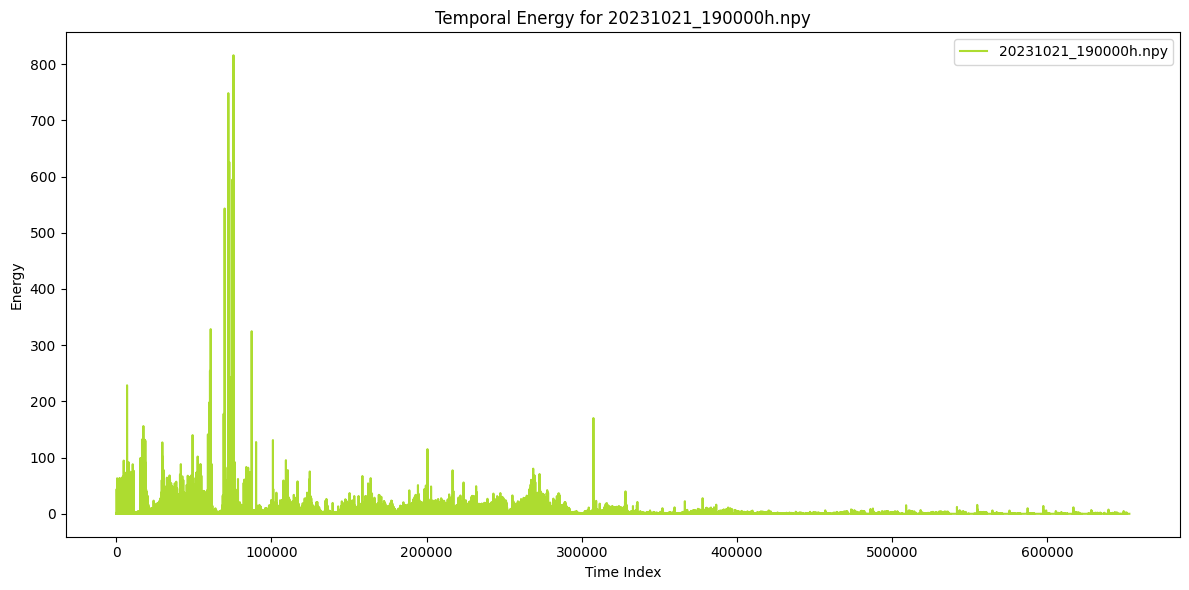
\includegraphics[width=\columnwidth]{assets/temp_energy.png}
    \caption{Energía Temporal del Audio \textbf{h}.}
    \label{fig:energy}
\end{figure}


\textbf{Preprocesado de los archivos de audio aplicando cortes de frecuencia.}\\

Para eliminar las bajas energías en cada audio, es decir, lo que se consideró ruido, se analizan los histogramas de las energías (Figura \ref{fig:hist}),
y se calcula el ancho del primer bin. Dicho ancho será el mínimo de energía que se tomará en cuenta para filtrar la información relevante.\\

\begin{figure}[h!]
    \centering
    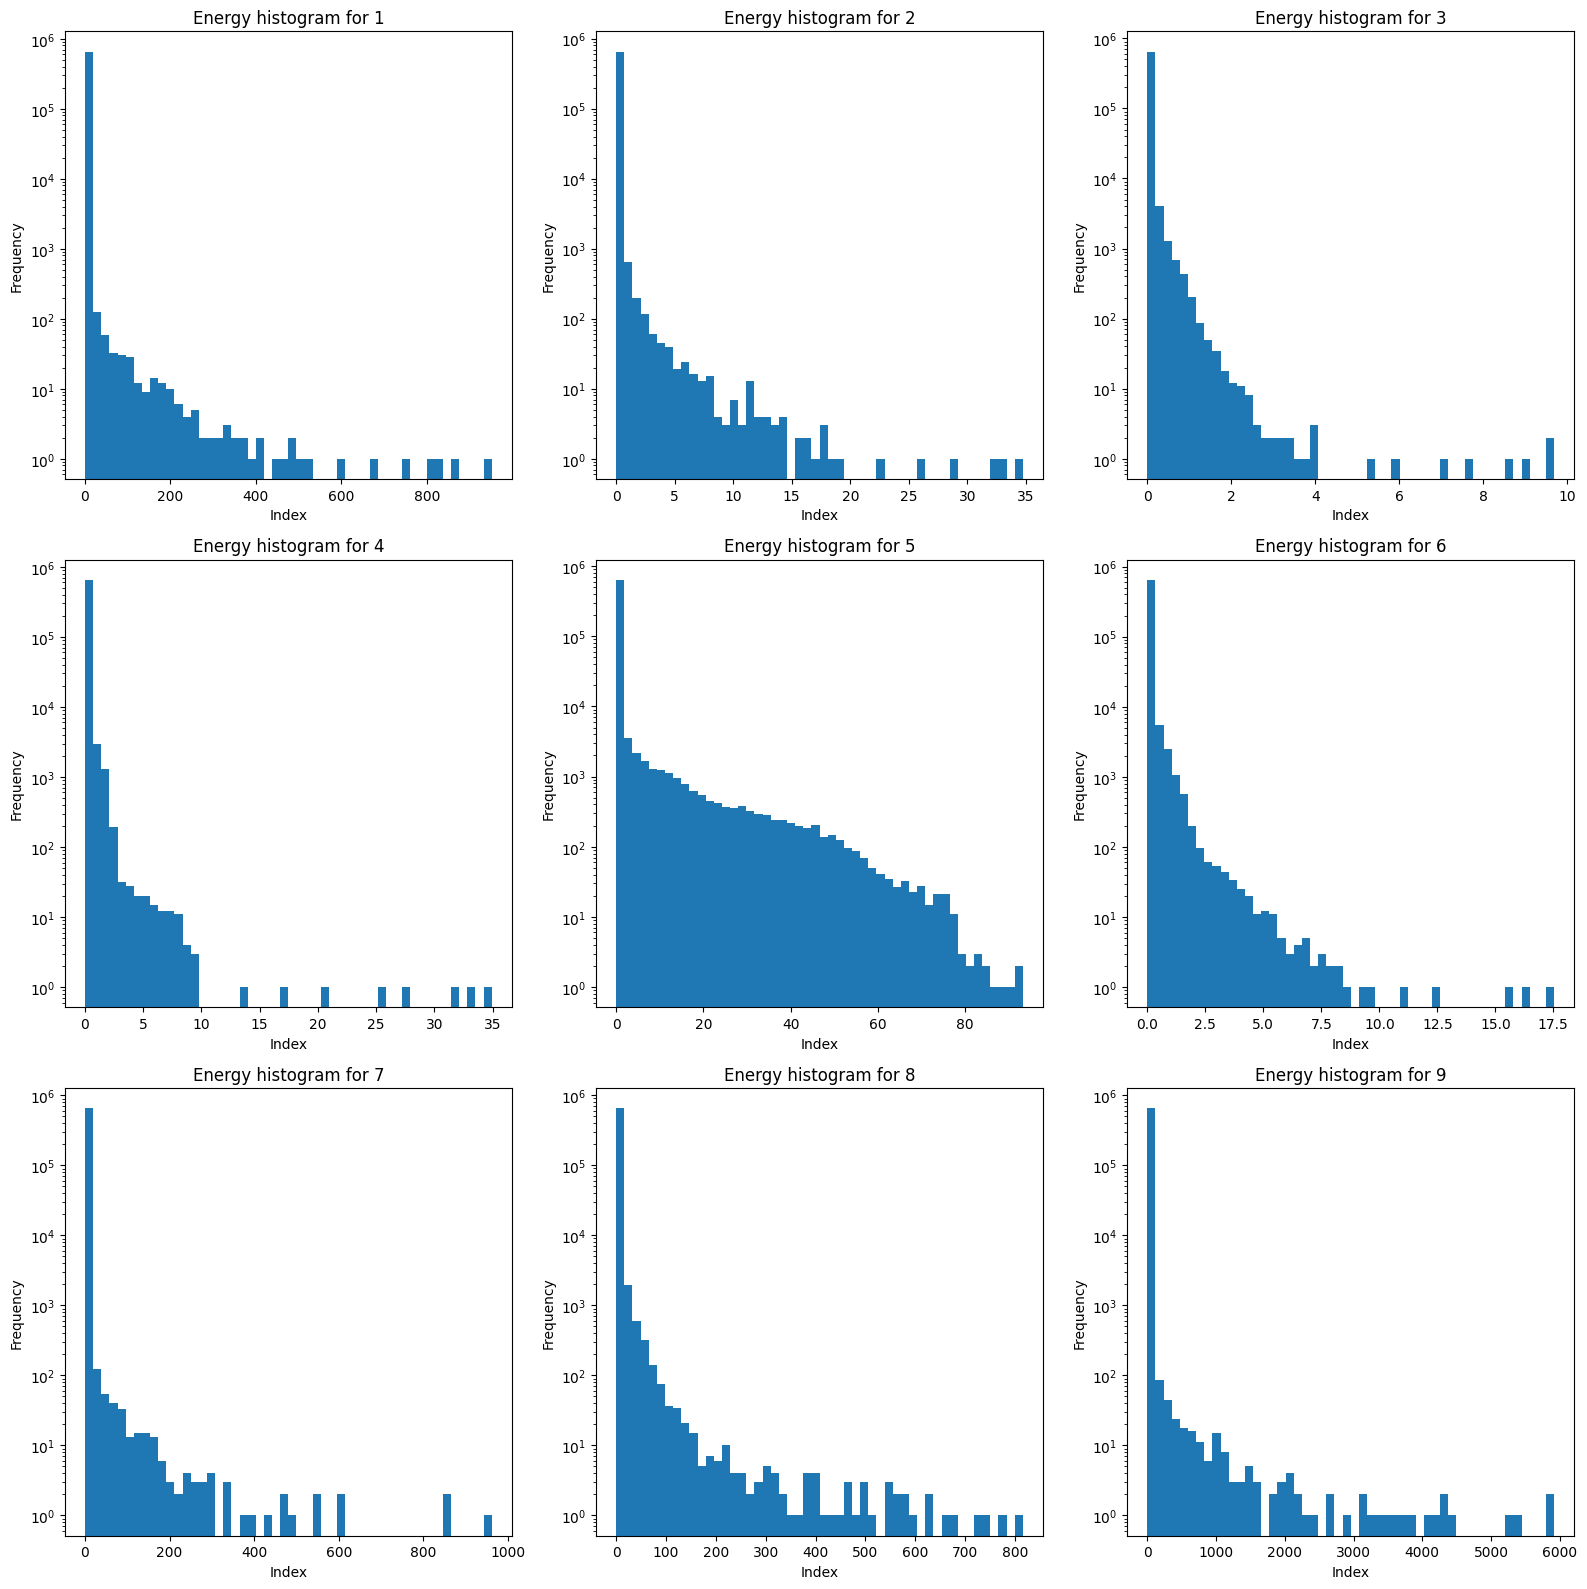
\includegraphics[width=\columnwidth]{assets/energy_hist.png}
    \caption{Histogramas de Frecuencias de las Energías Temporales de los Audios Filtrados por el Rango de Bandas Seleccionado.}
    \label{fig:hist}
\end{figure}


\textbf{Identificación de picos de energía en las señales.}\\

La obtención de los momentos de pico de energía se lleva a cabo utilizando
la función \textbf{find\_peaks} de la biblioteca \textbf{scipy.signal}.
Esta devuelve los índices en los que identifica un pico en la función que se le pasa.
En este caso se le pasa la función de energías temporales de cada audio una vez eliminado el ruido.
El resultado es como el que se muestra en la Figura \ref{fig:peaks}.\\

\begin{figure}[h!]
    \centering
    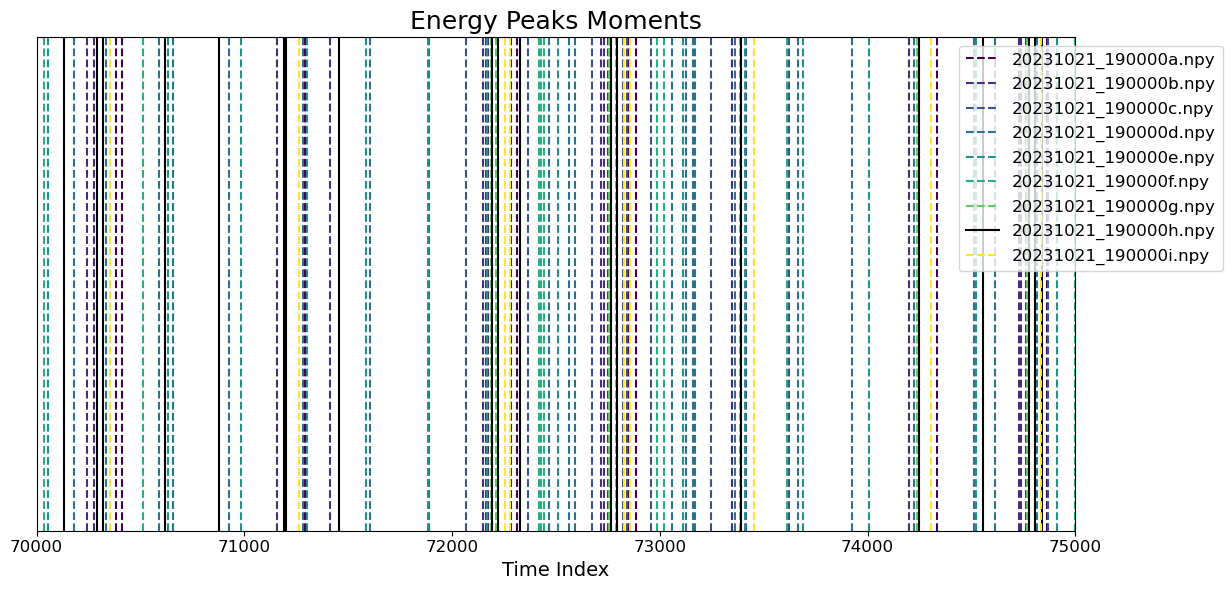
\includegraphics[width=\columnwidth]{assets/peaks_before.png}
    \caption{Momentos de Pico de Energía para un Fragmento de cada Audio.}
    \label{fig:peaks}
\end{figure}

\textbf{Cálculo de los desfases (\textit{lags}) entre los picos de los archivos y el archivo pivote mediante Correlación Cruzada.}\\

Luego se procede a calcular los desfases. Este método se basa en la suposición de que 
en el rango de frecuencias en el que una señal que sea captada por todos los audios de forma clara
se debe experimentar un máximo de energía en el mismo momento, por lo que sicrinizar los momentos de pico de 
energía es equivalente a sincronizar toda la información de los audios. La \textbf{Correlación Cruzada}
aplicada a un par de \textit{arrays} binarios cacula un coeficiente de coincidencias entre ambos, por lo que 
el \textit{lag} se calculó como el desfase que maximiza dicha coincidencia. El resultado se ve como en la Figura \ref{fig:peaksafter}.

\begin{figure}[h!]
    \centering
    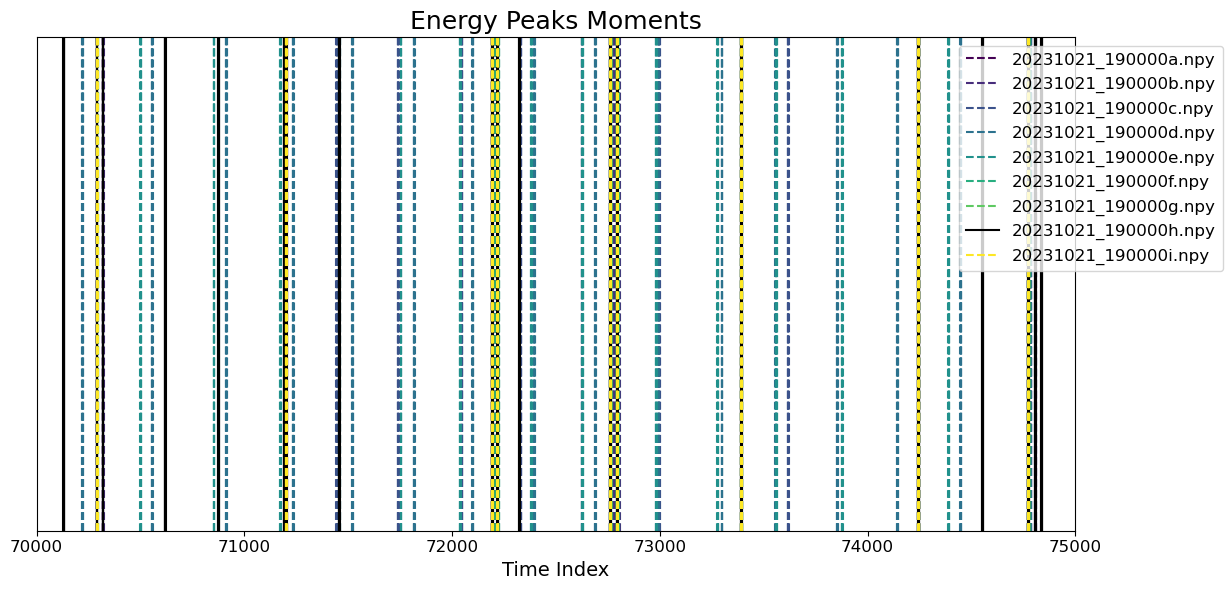
\includegraphics[width=\columnwidth]{assets/peaks_after.png}
    \caption{Momentos de Pico de Energía para un Fragmento de cada Audio después de Alinear.}
    \label{fig:peaksafter}
\end{figure}

\textbf{Aplicación de los desfases a los audios originales para su sincronización.}\\

Finalmente se aplican los desfases obtenidos a los archivos originales para comenzar con su procesamiento para la obtención de secuencias de cantos.\\



\textbf{Obtención de secuencias de cantos}\\

Para llevar a cabo esta parte del estudio, se consideró oportuno
separar la información de los archivos en CO y LIN, para 
realizar en paralelo los procesamientos en los momentos de baja y alta frecuencia respectivemente.
De forma análoga a como se hace en la sincronización, se calculan las
energías temporales y se establece un umbral de energía para
eliminar el ruido en cada audio. El método propuesto para identificar
el individuo más cercano a cada micrófono se sustenta en la suposición de que
para un micrófono, los cantos del individuo más cercano deben ser registrados con las
mayores energías relativas a dicho micrófono. Por lo tanto, si en cada uno se identifican 
las energías grandes y se elimina la información de esos cantos de las demás grabaciones,
se obtendrán por separado los datos que se buscan.
El algoritmo que representa lo antes expuesto consiste en lo siguiente:

\begin{itemize}
	\item Se guardan copias vacías (llenas de ceros) de los \textit{arrays} de energías temporales.
	\item Se selecciona de forma aleatoria uno de los 9 archivos. 
	\begin{itemize}
		\item En él se selecciona el índice donde se registra la energía máxima. 
		\item Si la energía es mayor que el umbral para el archivo seleccionado, se copia su valor en el índice del archivo vacío correspondiente.
		\item Se borra el valor que exista en dicho índice en los 9 archivos (se coloca un 0).
	\end{itemize}
	\item Se repite el proceso anterior hasta que en cada \textit{array} de energía temporal solo queden valores por debajo de su respectivo umbral.
	\item Finalmente se guardan los resultados.
\end{itemize}

Este proceso se repite una cantidad determinada de veces para comparar los resultados de corridas diferentes y comprobar su consistencia.\\


Luego de hecho esto, el resultado de la identificación de Elenas por micrófonos, visto como una secuencia general, se vería como en la Figura \ref{fig:seq}

\begin{figure}[h!]
    \centering
    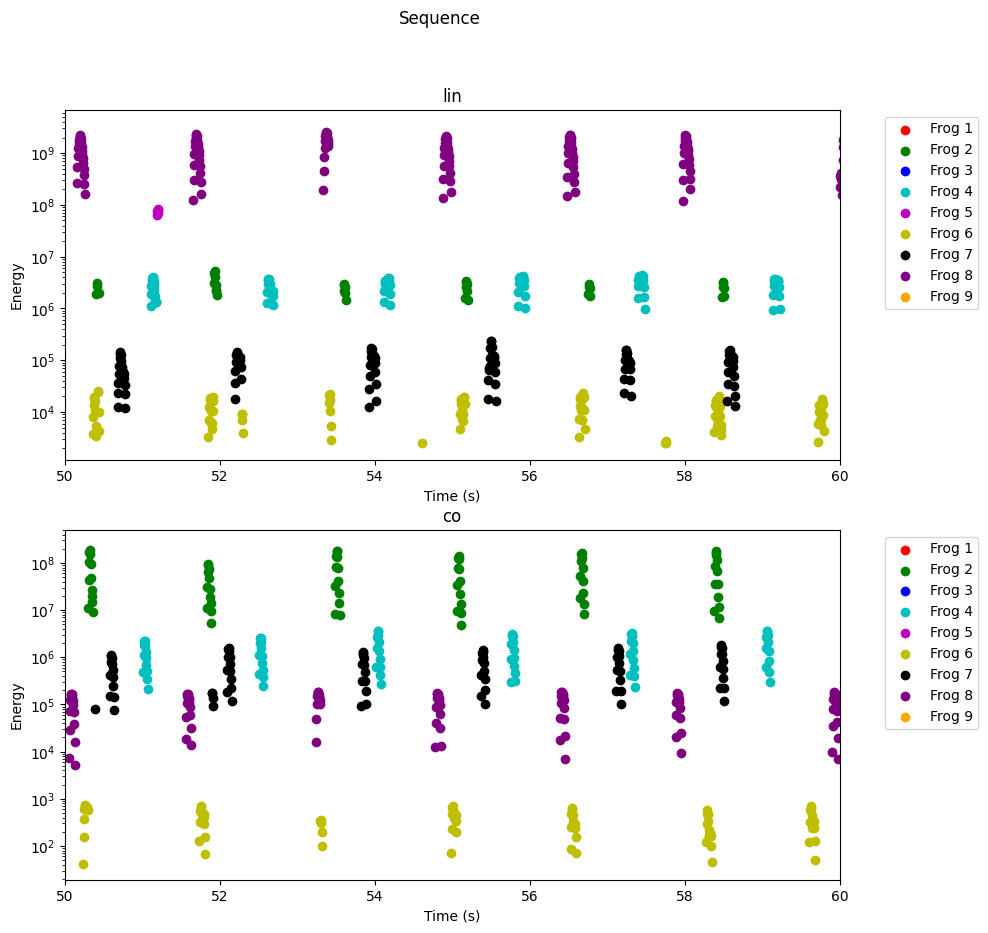
\includegraphics[width=\columnwidth]{assets/sequence.png}
    \caption{Fragmento de Secuencia de Cantos de las Elenas.}
    \label{fig:seq}
\end{figure}


Una vez identificada la secuencia de cantos de cada Elena, 
se analizó el comportamiento del coro en cuanto a las bandas de frecuencia.
De lo observado en las figuras \ref{fig:freqlin} y \ref{fig:freqco}
se puede formular la hipótesis de que las Elenas regulan la frecuencia de sus
cantos en dependencia de las frecuencias de los demás miembros del coro,
buscando baja superposición y tal vez mayor distinguibilidad.



\begin{figure}[h!]
    \centering
    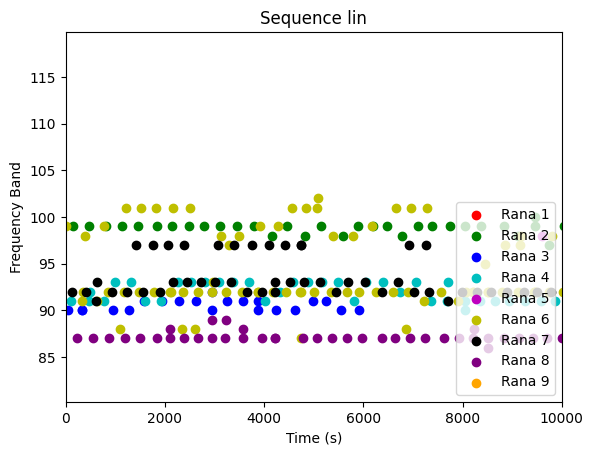
\includegraphics[width=\columnwidth]{assets/frequencylin.png}
    \caption{Comportamiento del Coro en Cuanto a la Frecuencia de los LIN.}
    \label{fig:freqlin}
\end{figure}

\begin{figure}[h!]
    \centering
    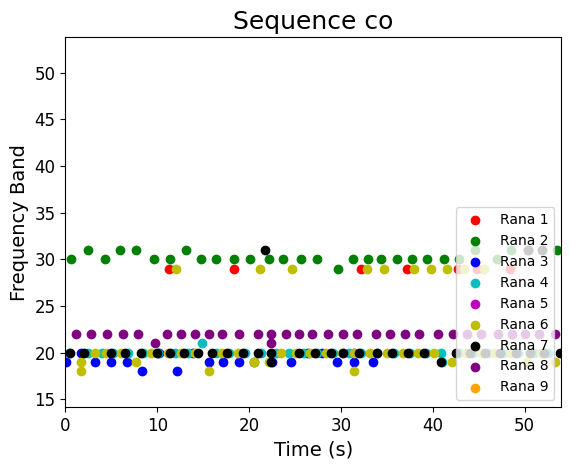
\includegraphics[width=\columnwidth]{assets/frequencyco.png}
    \caption{Comportamiento del Coro en Cuanto a la Frecuencia de los CO.}
    \label{fig:freqco}
\end{figure}

El análisis de dicha hipótesis, la estadística de los coros,
un estudio de causalidad, son algunas de las líneas futuras de esta investigación. 
El código fuente de este trabajo puede ser encontrado en el siguiente repositorio de GitHub:
\href{https://github.com/DanielMPMatCom/Identifying-Elenas.-JCE-MatCom.git}{Identifying Elenas. JCE MatCom}\\


Agradecimientos al Dr. Milton Borroto por su asesoria con la alineacion y deteccion de las ranas y al Dr. Roberto Alonso por sus consejos sobre el comportamiento de la especie y por proveernos de los datos.

\begin{thebibliography}{}
	
	\bibitem{elena} Alonso, R., Rodríguez-Gómez, A., \& Estrada, A. R. (2001). Patrones de actividad acústica y trófica de machos cantores de Eleutherodactylus eileenae (Anura: Leptodactylidae). Revista española de herpetología, 15(2001), 45-52.

	
	\bibitem{mel} Centic Murcia. (n.d.). Mel Spectogram. Curso de Ciencia de Datos. \href{https://centicmurcia.github.io/curso-ciencia-datos/3.6-audio/1\%20-\%20Mel\%20Spectogram/}{https://centicmurcia.github.io/curso-ciencia-datos/3.6-audio/1\%20-\%20Mel\%20Spectogram/}
	
	\sloppypar
	\bibitem{cross_corr} Bourke, P. (1996). Cross correlation. Cross Correlation”, Auto Correlation—2D Pattern Identification, 596.
  
	\bibitem{energy} Jurafsky, D., \& Martin, J. H. (2008). Speech and language processing (2nd ed., p. 304). Pearson.

\end{thebibliography}
	  


%===================================================================================


\label{end}

\end{document}

%===================================================================================
